% Tento soubor nahraďte vlastním souborem s obsahem práce.
%=========================================================================
% Autoři: Michal Bidlo, Bohuslav Křena, Jaroslav Dytrych, Petr Veigend a Adam Herout 2019

% Pro kompilaci po částech (viz projekt.tex), nutno odkomentovat a upravit
%\documentclass[../projekt.tex]{subfiles}

%\newenvironment{definice}{\begin{quote}\textbf{Definice:}}{\end{quote}}

\newtheorem{definition}{Definice}
\newtheorem{remark}{Pozn\'amka}
\newtheorem{example}{Příklad}
\newtheorem{graph}{Obr\' azek}
\newtheorem{sentence}{Věta}
\newtheorem{tabul}{Tabulka}
%\newcommand{\comment}[1]{}

\chapter{Úvod}

\color{blue} Pár vět, které pak chci zakomponovat do \'uvodu nějak:
                \\ 
                \color{black} Zatímco bivalenční logika pracuje s binárními hodnotami "pravda" a "nepravda", fuzzy logika umožňuje pracovat s hodnotami, které se pohybují mezi těmito extrémy.






\chapter {Fuzzy mno\v ziny a fuzzy logika}
\section{Fuzzy mno\v ziny} 

%\comment{
%V klasické i fuzzy logice se často setkáváme se základními pojmy množina a prvek množiny. Množina se obecně %vysvětluje jako souhrn, soubor nebo skupina objektů. Tyto objekty pak nazýváme prvky dané množiny. Nejvíce %charakteristická vlastnost množin je, že je jednoznačně určena svými prvky, ale ignoruje jejich pořadí a %další jejich struktury. Množina, která neobsahuje žádné prvky, se nazývá prázdná množina.
%}

V běžném životě se často setkáváme s nepřesnými pojmy, jako jsou např. \clqq málo\crqq, \clqq hodně\crqq \space či třeba \clqq trochu\crqq \space. Jak ale takovou vágnost vyjádřit v matematice? Pokud člověk vyjádří výrok, že je \clqq celkem mladý\crqq, znamená to, že je mladý nebo ne? K zápisu a práci s takovými výroky se pak ve fuzzy logice využívají fuzzy množiny a operace s nimi.

Nech\v t je např. vypsáno výběrové řízení modelingové agentury s požadavkem, že hledají vysoké uchazeče. Taková informace je tedy poněkud vágní, ačkoliv v běžném životě lehce srozumitelná. Pokud by se někdo pokusil definovat pojem \clqq vysoký člověk\crqq \space pomocí ostré množiny, musel by nejprve stanovit hranici, kdy je člověk vysoký, např. 180 centimetr\r u, množina všech vysokých lidí V by měla charakteristickou funkci

    $$\chi_V:(x)=\begin{cases} 1, & \mbox{pokud }  x \geq 180,\\    0, & \mbox{pokud } x < 180,  \end{cases}$$

    čímž by došlo k paradoxu, že člověk který má 179,9 centimetr\r u je považován za nízkého a člověk se 180 centimetry za vysokého.

    Takový problém je zp\r usoben tím, že byla výška modelována jako vlastnost, kterou m\r uže mít člověk pouze v nulové míře nebo na 100\%. Za určitě vysokého člověka byl považován někdo se 180 centimetry, 175 centimetr\r u vysoký člověk byl podle stejného přístupu určitě malý. Přičemž 175 centimetr\r u vysoký člověk je běžně považován do určité míry za vysokého. Přesně z toho d\r uvodu se zavedl pojem \textit{fuzzy množina}, která náleží tzv. \textit{univerzu}. \textit{Univerzum} $X \in [0,\infty[$ teoreticky znamená množinu veškerých možných výšek všech lidí. Množina všech možných zájemc\r u je pak vyjádřitelná jako podmnožina $A$ univerza $X.$
    \begin{definition}
    \cite{navara}
        Fuzzy podmnožina univerza X (stručně fuzzy množina) je objekt A, který popisuje (zobecněná) charakteristická funkce (funkce příslušnosti) $\mu: X \rightarrow [0,1]$. Obor pravdivostních hodnot: $R(A) = \{\alpha \in [0,1]: (\exists x \in X : \mu_A(x) = \alpha)\} = \mu_A(X)$
    \end{definition}
    Fuzzy množina nebo také neostrá množina je pak množina prvků takových, jejichž afiliace je k této množině odstupňovaná. Fuzzy množina staví na stejných pravidlech, jako klasická booleovská množina, s tím rozdílem, že příslušnost nemusí nabývat jen hodnot 0 a 1, ale jakoukoliv hodnotu z intervalu [0,1]. 
    
    Ve fuzzy matematice se dále zavedl pojem funkce příslušnosti.
    \begin{definition}
        \cite{Kolo} Funkce příslušnosti fuzzy množiny A na (ostré) množině X: $\mu_A : X \rightarrow  [0,1].$ Stupe\v n příslušnosti x $\in A$ tedy m\r uže být libovolné číslo $\alpha \in [0,1]$.
    \end{definition}
    Funkce příslušnosti umož\v nuje vyjádřit částečnou příslušnost k množinám na intervalu [0,1], tedy jak moc lze označit pojem za \clqq pravdu\crqq \space či \clqq nepravdu\crqq. Díky čemuž se pak dají matematicky vyjádřit vágní pojmy jako \clqq docela dost\crqq, \clqq málo\crqq \space nebo \clqq mnoho\crqq \space apod.

     Pokud by se v předchozím zmíněném výběru modelingové agentury označila výška 180 centimetr\r u stupněm vlastnosti \clqq vysoký\crqq \space 1, pak je možné přiřadit výšce 175 cemtimetr\r u například stupe\v n 0,85. Když je každému prvku $x$ ze základního prostoru [0, $\infty$[ přiřazeno číslo z intervalu [0,1], které vyjadřuje míru, ve které je člověk mající výšku $x$ vysoký, lze pak získat funkci, která kompletně charakterizuje pojem vysoký člověk: $\mu_V: \Omega \rightarrow [0,1]$, kde $\Omega = [0, \infty[$ vyjadřuje základní prostor neboli univerzum. Takovou funkcí je např. funkce $\mu_V:  [0, \infty[ \rightarrow [0,1]$, 

    $$\mu_V:(x)=\begin{cases} 1, & \mbox{pokud }  x \geq 180,\\ 
    \frac{x}{20} - 8, & \mbox{pokud } 160 \leq x \leq 180,\\
    0, & \mbox{pokud } x < 160,  \end{cases}$$

    jíž graf je vykreslen níže.

    \begin{graph} Graf funkce příslušnosti fuzzy množiny V - \clqq Vysoký člověk\crqq.\\
        \begin{tikzpicture}
        \hspace*{2cm}
            \begin{axis}[
                xlabel=$x$, % Popisek osy x
                ylabel=$y$, % Popisek osy y
                axis lines=middle, % Zobrazení os
                ymin=0, ymax=1.2, % Rozsah osy y
                xmin=0, xmax=250, % Rozsah osy x
                xtick={0, 160, 180}, % Označení na ose x
                ytick={ 0, 0.8, 1}, % Označení na ose y
                legend style={at={(0.5,-0.2)}, anchor=north},
                width=10cm, % Šířka grafu
                height=6cm, % Výška grafu
                grid=both, % Zobrazení mřížky
                grid style={line width=0.2pt, draw=gray!30},
            ]
            
            % Definice prvního segmentu
            \addplot[blue, ultra thick, domain=180:250, samples=100] {1};
            
            % Definice druhého segmentu
            \addplot[blue, ultra thick, domain=160:180, samples=100] {x/20 - 8};
             \addlegendentry{V}
            
            % Definice třetího segmentu
            \addplot[blue, ultra thick, domain=0:160, samples=100] {0};
            
            \end{axis}
        \end{tikzpicture}
    \end{graph}



Pokud bychom chtěli modelovat funkci příslušnosti odlišného fuzzy výroku, např. výroku \clqq asi 3\crqq, lze zvolit několik možných řešení tohoto problému. Každý pak vyjadřuje jiný rozptyl možných řešení.
\begin{graph} Grafické znázornění funkcí příslušnosti výroku P \clqq asi 3\crqq.\\


    \resizebox{5.27cm}{!}{%zde se meni velikost grafu
                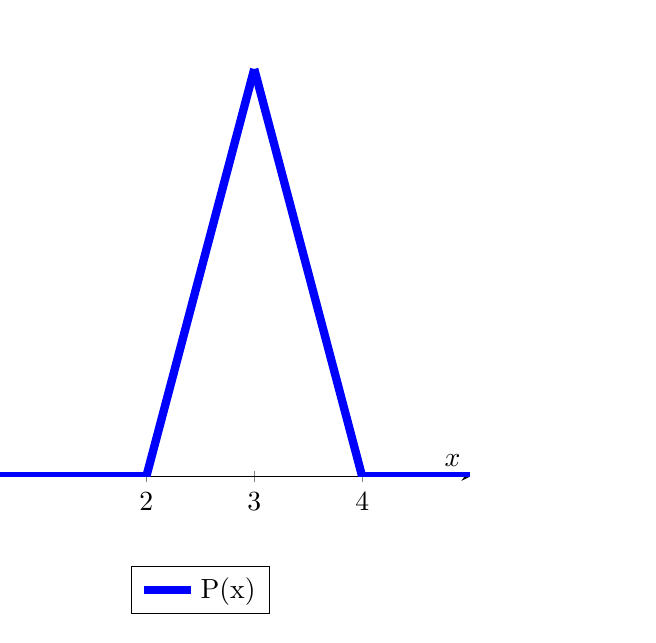
\begin{tikzpicture}
                \hspace*{-2cm}
                	\begin{axis}[
                        axis lines=middle,
                        xlabel=$x$,
                        ylabel=$y$,
                        xtick={0, 2, 3, 4}, % Označení na ose x
                        ytick={ 0, 0.5, 0.8, 1}, % Označení na ose y
                        legend style={at={(0.5,-0.2)}, anchor=north},
                        xmin=0, xmax=5, 
                        ymin=0, ymax=1.1,
                    ]
                    
                    \addplot[blue, domain=0:3, line width = 3pt] {x-2};
                    \addlegendentry{P(x)}
                    
                    \addplot[blue, domain=3:5, line width = 3pt,] {-x + 4};
                    \addplot[blue, domain=4:5, line width = 3pt,] {0};
                    \addplot[blue, domain=0:2, line width = 3pt,] {0};

                	\end{axis}
                \end{tikzpicture}
            }
    \resizebox{5.27cm}{!}{%zde se meni velikost grafu
                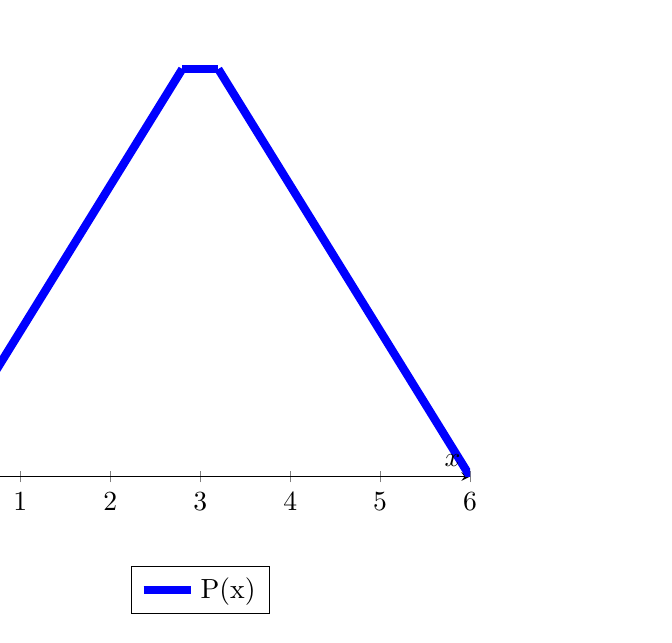
\begin{tikzpicture}
                \hspace*{-2cm}
                	\begin{axis}[
                        axis lines=middle,
                        xlabel=$x$,
                        ylabel=$y$,
                        xtick={0, 1, 2, 3, 4, 5, 6}, % Označení na ose x
                        ytick={ 0, 0.5, 0.8, 1}, % Označení na ose y
                        legend style={at={(0.5,-0.2)}, anchor=north},
                        xmin=0, xmax=6, 
                        ymin=0, ymax=1.1,
                    ]
                    
                    \addplot[blue, domain=0:2.8, line width = 3pt] {x/2.8};
                    \addlegendentry{P(x)}
        
                    \addplot[blue, domain=2.8:3.2, line width = 3pt,] {1};
                    \addplot[blue, domain=3.2:6, line width = 3pt,] {-5*x/14 + 15/7};

                	\end{axis}
                \end{tikzpicture}
            }
    \resizebox{5.27cm}{!}{%zde se meni velikost grafu
                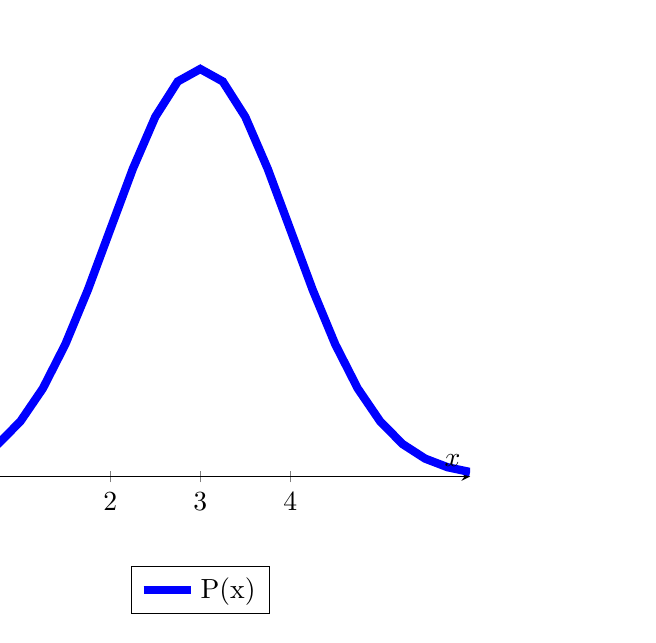
\begin{tikzpicture}
                \hspace*{-2cm}
                	\begin{axis}[
                        axis lines=middle,
                        xlabel=$x$,
                        ylabel=$y$,
                        xtick={0, 2, 3, 4}, % Označení na ose x
                        ytick={ 0, 0.5, 0.8, 1}, % Označení na ose y
                        legend style={at={(0.5,-0.2)}, anchor=north},
                        xmin=0, xmax=6, 
                        ymin=0, ymax=1.1,
                    ]
                    
                    \addplot[blue, domain=0:6, line width = 3pt] {exp(-(x-3)^2/2)};
                    \addlegendentry{P(x)}


                	\end{axis}
                \end{tikzpicture}
            }
\end{graph}



\section{Fuzzy logick\'e spojky}
Fuzzy logické spojky n\'am umožňují vyjádřit vágnost a neurčitost v logických operacích. Tyto spojky se často využívají v aplikacích jako jsou řízení průmyslových procesů, rozpoznávání vzorů, vývoj umělé inteligence a dalších oblastech, kde je potřeba pracovat s neurčitými informacemi.\\

V\v sechny fuzzy logick\'e spojky jsou monot\'onn\'im roz\v s\'i\v ren\'im klasick\'ych logick\'ych spojek. Na dalších kapitolách budou postupně představeny základní fuzzy spojky, mezi kter\'e  patří 
fuzzy negace, konjunkce, disjunkcie a implikace. 

\subsection{Fuzzy negace}

Fuzzy negace představují klíčový koncept v oblasti fuzzy logiky. Tyto negace jsou zobecn\v en\'im klasick\'ych negac\'i. Základní vlastnosti fuzzy negací jsou:

\begin{enumerate}
\item \textbf{Soudržnost:}\\
Pro hodnoty $0$ a $1$ se fuzzy negace shoduje s klasickou negac\'i.
    \item \textbf{Kontinuita hodnot:} \\
        Fuzzy negace nepracuje jenom s  ostrými hodnotami „pravda“ a „nepravda“, ale na stupni neurčitosti či specifickým číselném zápisu, který reflektuje stupeň nepravdivosti.
    \item \textbf{Monotonie:} \\
        Fuzzy negace jsou monot\'onn\'im roz\v s\'i\v ren\'im klasick\'e negace, což znamená, že s rostoucími vstupn\'imi hodnotami klesaj\'i hodnoty výstupn\'e.
    
\end{enumerate}

\begin{definition}
\cite{Kolo} Fuzzy negací nazýváme každou funkci $N:[0, 1] \to [0, 1]$  s vlastnostmi:
    \begin{enumerate}
        \item  $N(0) = 1, N(1) = 0,$
        \item $\forall  x, y \in [0, 1]: x < y \Rightarrow{} N(x) \geq N(y).$
     \end{enumerate}
\end{definition}
     \begin{example}
         Funkce $N_S(x)=1-x$ spl\v nuje vlastnosti fuzzy negace na intervalu $[0,1].$ Je to nejzn\'am\v ej\v s\'i fuzzy negace, kterou ve sv\'e pr\'aci p\v redstavil Lotfi A. Zadeh a obvykle je ozna\v cov\'ana jako standardn\'i negace.   Fuzzy negace nemus\'i b\'yt nutn\v e spojit\'a funkce. Zn\'am\'e p\v r\'iklady nespojit\'ych fuzzy negac\'i jsou n\'asleduj\'ic\'i funkce:
         $$ N_{\bot}(x)=\begin{cases} 1, & \mbox{pokud }x=0, \\
         0, & \mbox{pokud }x\in \mbox{]0, 1]}, \end{cases} 
         N_{\top}(x)=\begin{cases} 1, & \mbox{pokud }x\in \mbox{[0, 1[}, \\
         0, & \mbox{pokud }x=1. \end{cases}$$
         Funkce $N_{\bot}$ je nejmen\v s\'i a funkce $N_{\top}$ je nejv\v et\v s\'i fuzzy negace, proto
         \begin{equation}
        N_{\bot}(x) \geq N(x) \geq N_\top(x)  \mbox{ pro každé } x \in [0, 1]. \
    \end{equation}
    V literatu\v re jsou negace $N_\bot, N_\top$ zn\'am\'e jako Gödelovy fuzzy negace.
    
    Funkce $N_1(x) = \sqrt{1-x}$ a $N_2(x) = \sqrt{1-x^2}$ jsou zřejmě pro $ x \in [0,1]$ nerostoucí a tak\'e plat\'i:
        \begin{enumerate}
            \item $N_1(0) = \sqrt{1-0} = 1, 
                    N_1(1) = \sqrt{1-1} = 0, $
            \item $N_2(0) = \sqrt{1-0^2} = 1,
                    N_2(1) = \sqrt{1-1^2} = 0.$
        \end{enumerate}
         Tedy i tyto funkce jsou fuzzy negace.

         \begin{graph} Grafy dříve zmíněných funkcí $N_s$, $N_{\bot}$,$ N_{\top}$, $N_1$ a $N_2.$\\
         \\
            \resizebox{150pt}{!}{%zde se meni velikost grafu
                \begin{tikzpicture}
                \hspace*{-2cm}
                	\begin{axis}[
                        axis lines=middle,
                        xlabel=$x$,
                        ylabel=$y$,
                        xmin=0, xmax=1.1, 
                        ymin=0, ymax=1.1, 
                        legend entries={$N_s$ = $1-x$},
                        legend style={at={(0.5,-0.2)}, anchor=north}
                    ]
                		\addplot[samples = 500,
                            	smooth,
                            	ultra thick,
                            	blue,] {1-x};
    
                	\end{axis}
                \end{tikzpicture}
            }
            \resizebox{150pt}{!}{%zde se meni velikost grafu
                \begin{tikzpicture}
                \hspace*{-1cm}
                	\begin{axis}[
                        axis lines=middle,
                        xlabel=$x$,
                        ylabel=$y$,
                        xmin=0, xmax=1.1, 
                        ymin=0, ymax=1.1, 
                        %xtick={-1,0,1,2},
                        %ytick={-0.5,0,1,1.5},
                        legend entries={$N_{\bot}(x)$},
                        legend style={at={(0.5,-0.2)}, anchor=north}
                    ]
                    
                    % Prvý prípad: g(x) = 1 pre x = 0
                    \addplot[blue, mark=*] coordinates {(0, 1)};
                    
                    % Druhý prípad: g(x) = 0 pre 0 < x < 1
                    \addplot[blue, domain=0:1, samples=100, line width = 3pt,] {0};

                    \addplot[only marks, mark=*, mark size=3pt, mark options={fill=white}] coordinates {(0, 0)};
    
                	\end{axis}
                \end{tikzpicture}
            }
            \resizebox{150pt}{!}{%zde se meni velikost grafu
                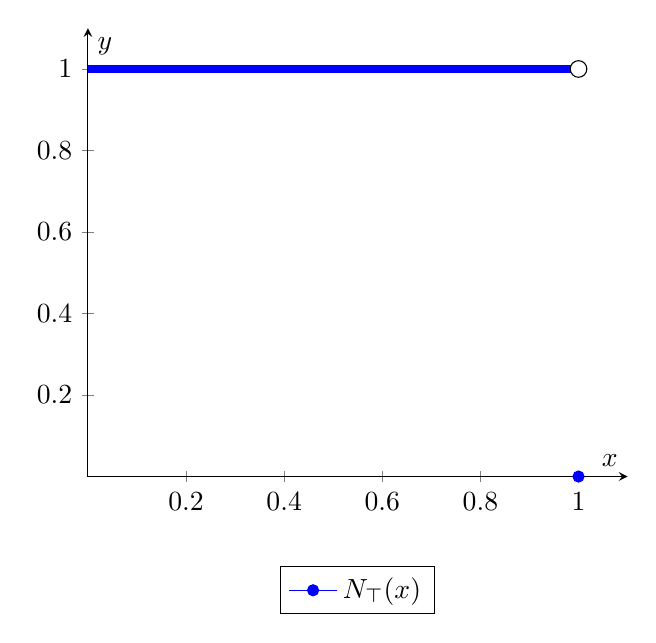
\begin{tikzpicture}
                \hspace*{0cm}
                	\begin{axis}[
                        axis lines=middle,
                        xlabel=$x$,
                        ylabel=$y$,
                        xmin=0, xmax=1.1, 
                        ymin=0, ymax=1.1, 
                        %xtick={-1,0,1,2},
                        %ytick={-0.5,0,1,1.5},
                        legend entries={$N_{\top}(x)$},
                        legend style={at={(0.5,-0.2)}, anchor=north}
                    ]
                    
                    % Prvý prípad: g(x) = 1 pre x = 0
                    \addplot[blue, mark=*] coordinates {(1, 0)};
                    
                    % Druhý prípad: g(x) = 0 pre 0 < x < 1
                    \addplot[blue, domain=0:1, samples=100, line width = 3pt,] {1};

                    \addplot[only marks, mark=*, mark size=3pt, mark options={fill=white}] coordinates {(1, 1)};
    
                	\end{axis}
                \end{tikzpicture}
            }

            \resizebox{150pt}{!}{%zde se meni velikost grafu
                \begin{tikzpicture}
                \hspace*{2cm}
                	\begin{axis}[
                        axis lines=middle,
                        xlabel=$x$,
                        ylabel=$y$,
                        xmin=0, xmax=1.1, 
                        ymin=0, ymax=1.1, 
                        %xtick={-1,0,1,2},
                        %ytick={-0.5,0,1,1.5},
                        legend entries={$N_1$ = $\sqrt{1-x}$},
                        legend style={at={(0.5,-0.2)}, anchor=north}
                    ]
                	\addplot[samples = 200,
                            domain=0:1,
                        	smooth,
                        	ultra thick,
                        	blue,] {sqrt(1-x)};
    
                    
                	\end{axis}
                \end{tikzpicture}
            }
            \resizebox{175pt}{!}{%zde se meni velikost grafu
                \begin{tikzpicture}
                \hspace*{3cm}
                	\begin{axis}[
                        axis lines=middle,
                        xlabel={$x$},
                        ylabel={$y$},
                        xmin=0, xmax=1.1, 
                        ymin=0, ymax=1.1, 
                        xtick={0,0.2,0.4,0.6,0.8,1},
                        ytick={0,0.2,0.4,0.6,0.8,1},
                        legend entries={$N_2$ = $\sqrt{1-x^2}$},
                        legend style={at={(0.5,-0.2)}, anchor=north}
                    ]
                	\addplot[samples = 200,
                            domain=0:1,
                        	smooth,
                        	ultra thick,
                        	blue,] {sqrt(1-x^2)};
    
                   
                	\end{axis}
                \end{tikzpicture}
            }
        \end{graph}
    \end{example}

   N\v ekter\'e fuzzy negace maj\'i dal\v s\'i zaj\'imav\'e vlastnosti:

    \begin{definition}
    \cite{Kolo}
        Kdy\v z $N: [0,1] \to [0,1]$ je klesající a spojitá fuzzy negace, \v r\'ik\'ame, \v ze $N$ je striktní negace.
        Striktn\'i fuzzy negace, kter\'a je involutivní, tedy, pro kterou plat\'i $N(N(x)) = x $ pro každé $ x \in [0,1]$, se nazývá silná fuzzy negace.
    \end{definition}

    \begin{example}
        Spojit\'e neg\'atory $N_S, N_1, N_2$ z p\v redchoz\'iho p\v rikladu jsou evidetn\v e striktn\'i, proto\v ze jsou ryze monot\'onn\'i. D\'ale plat\'i:
        $$N_S(N_S(x))=1-(1-x)=x, \mbox{pro ka\v zd\'e } x \in [0,1],$$
                $$N_1(N_1)) = N_1(\sqrt{1-x}) = \sqrt{1-\sqrt{1-x}} \neq x, \mbox{ pro každé } x \in ]0,1[,$$ $$N_2(N_2) = N_2(\sqrt{1-x^2}) = \sqrt{1-(\sqrt{1-x^2})^2} = x,
                \mbox{pro každé } x \in [0,1].$$
Takže negace $N_S$ a $N_2$ jsou involutivní a tím pádem tak\'e siln\'e negace, naopak
            negace $N_1$ není involutivní, tedy ani siln\'a fuzzy negace.
                
            \end{example}

    \begin{remark}
        Z rovnosti $N(N(x))=x$ plyne pro bijektivn\'i funkce tak\'e rovnost $N(x)=~N^{-1}(x).$ 
         Grafick\'a interpretace  t\'eto rovnosti  pro fuzzy negace je taková, že grafy involutivních fuzzy negací jsou osově souměrné podle osy $y = x$.
        \begin{graph} Ukázka osové souměrnosti bijektivní funkce f(x) = $\sqrt{1-x^2}$ podle osy y = x pro $x \in [0,1]$.\\
            
            \begin{tikzpicture}
            \hspace*{3cm}
            	\begin{axis}[
                        width=8cm,  % Nastavte požadovanou šířku grafu
                        height=8cm,
                        axis lines=middle,
                        xlabel=$x$,
                        ylabel=$y$,
                        xmin=0, xmax=1, 
                        ymin=0, ymax=1, 
                        %xtick={-1,0,1,2},
                        %ytick={-0.5,0,1,1.5},
                        legend entries={$g(x)$},
                        legend style={at={(0.5,-0.2)}, anchor=north}
                    ]
            		\addplot[samples = 500,
                        	smooth,
                        	very thick,
                        	blue,
                                domain=0:1,] {(1-x^2)^0.5};
                    \addplot[smooth,
                            	thin,
                            	red,
                            	dashed
                            ]  {x};
                \legend{y = $\sqrt{1-x^2}$, 
                    	y = x
                    }
            	\end{axis}
            \end{tikzpicture}
        \end{graph}
    \end{remark}


    
\subsection{Fuzzy konjunkce}

Fuzzy konkjunkce se využívají pro spojení dvou a více podmínek s ohledem na jejich vágnost a neostrost. Místo výsledného \clqq ano\crqq \space nebo \clqq ne\crqq \space je použita hodnota $x$, $x \in [0,1]$, která reprezentuje, do jaké míry jsou podmínky splněny.  
Základní vlastnosti fuzzy konjunkcí jsou:
\begin{enumerate}
    \item \textbf{Soudržnost:}\\
    Pro hodnoty 0 a 1 se fuzzy konjunkce shoduje s klasickou konjunkcí.
    \item \textbf{Kontinuita hodnot:}\\
    Fuzzy konjunkce nepracuje jenom s  ostrými hodnotami „pravda“ a „nepravda“, ale na stupni neurčitosti či specifickým číselném zápisu, který reflektuje stupeň pravdivosti.
    \item \textbf{Monotonie:}\\
    Fuzzy konjunkce je monotonní operace, tedy pokud A$\leq$ B$\leq$ C$\leq$ D, pak A$\land$B$\leq$ C$\land$D, což znamená, že s rostoucími vstupními hodnotami rostou i výsledky jejich konjunkce.
\end{enumerate}
\begin{definition}
    \cite{hlinena}
    Neklesající zobrazení C: $[0,1]^2 \rightarrow [0,1]$ se nazývá konjunktor, pokud pro libovolné a,b $\in$ [0,1] platí
    C(a,b) = 0 pokud a = 0, nebo b = 0,
    C(1,1) = 1.
    \end{definition}

\begin{remark}
    Fuzzy konjunkce mohou být modelovány pomocí triangulárních norem, kterým je věnována celá následující podkapitola.
\end{remark}

\subsection{Triangul\'arn\'i normy} 

Jak již bylo zmíněno, fuzzy konjunkce mohou být modelov\' any pomocí triangulárních norem, zjednodušeně t-norem. 
\begin{definition}
\cite{hlinena}
    Triangulární norma je binární operace na jednotkovém intervale [0,1], t.j. funkce $T: [0,1]^2 \rightarrow [0,1]$ taková, že pro každé $x, y, z \in [0,1]$ jsou splněné následující axiomy:
    \begin{enumerate}
        \item \textbf{Komutativnost:} $T(x,y) = T(y,x)$,
        \item \textbf{Asociativita:} $T(x, T(y, z)) = T(T(x, y), z)$,
        \item \textbf{Monotónnost:} pokud $y \geq z$ pak $T(x, y) \geq T(x, z)$,
        \item \textbf{Okrajová podmínka:} $T(x, 1) = x$.
    \end{enumerate}
\end{definition}

\begin{remark}
    Funkce je t-norma v případě, že spl\v nuje alespo\v n 3 ze 4 axiom\r u popsaných výše.
\end{remark}

\begin{example} Na několika příkladech jsou uvedeny funkce, které vždy spl\v nují 3 ze 4 axiom\r u.\\
    Funkce $F_1 : [0, 1]^2 \rightarrow [0, 1]$ daná přepisem\\
    $$F_1(x,y) = 13,$$
    spl\v nuje axiomy 1., 2., 3., ale nespl\v nuje axiom 4.\\

    Funkce $F_2 : [0, 1]^2 \rightarrow [0, 1]$ daná přepisem\\
    $$F_2(x,y) = x.y.max(x,y)$$
    spl\v nuje axiomy 1., 3., 4., ale nespl\v nuje axiom 2.\\

    Funkce $F_2 : [0, 1]^2 \rightarrow [0, 1]$ daná přepisem\\
    $$F_2(x,y) = x$$
    spl\v nuje axiomy 2., 3., 4., ale nespl\v nuje axiom 1.\\
    
\end{example}

Mezi základní triangulární normy se řadí minimová, součinová, Łukasiewiczova t-norma a drastický součin.
\begin{example}
\cite{hlinena}
    \begin{enumerate}
    \item \textbf{Minimová t-norma} $T_M: [0,1]^2 \rightarrow [0,1]$
    $$T_M(x,y) = min(x,y).$$
    \item \textbf{Součinová t-norma} $T_P: [0,1]^2 \rightarrow [0,1]$
    $$T_P(x,y) = x.y.$$
    \item \textbf{Łukasiewiczova t-norma} $T_L: [0,1]^2 \rightarrow [0,1]$
    $$T_L(x,y) = max(x+y-1,0).$$
    \item \textbf{Drastický součin} $T_D: [0,1]^2 \rightarrow [0,1]$
    $$T_D:(x)=\begin{cases} min(x,y), & \mbox{pokud }  max(x,y) = 1,\\ 
    0, &  jinak.  \end{cases}$$
\end{enumerate}
\end{example}

\begin{graph} Minimová t-norma $T_M$, Součinová t-norma $T_P$, Łukasiewiczova t-norma $T_L$, Drastický součin $T_D$.\\

   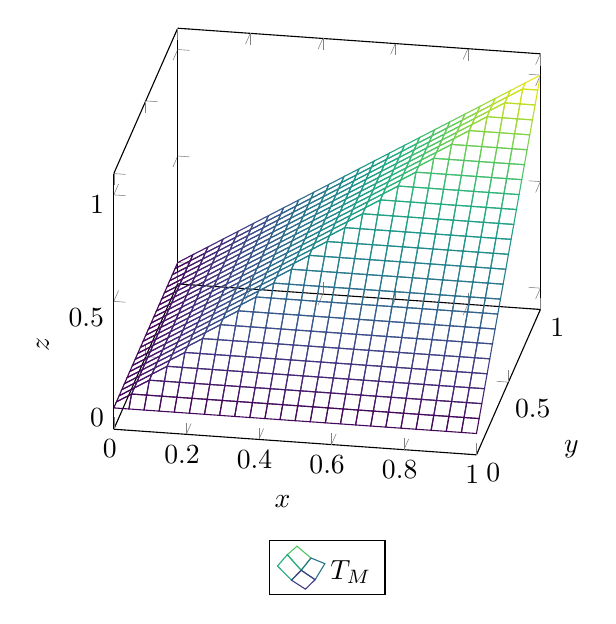
\begin{tikzpicture}
        \begin{axis}[
            width=7cm,  % Nastavte požadovanou šířku grafu
            height=7cm, % Nastavte požadovanou výšku grafu
            xlabel=$x$,
            ylabel=$y$,
            zlabel=$z$, % Popisek osy z
            domain=0:1, % Rozsah hodnot x
            y domain=0:1, % Rozsah hodnot y
            colormap/viridis, % Barevná mapa (nastavitelná)
            view={10}{30}, % Náhled na graf (úhel pohledu)
            legend style={at={(0.5,-0.2)}, anchor=north}
        ]
        
         \addplot3 [surf, shader=interp, mesh] {min(x,y)};
         \legend{$T_M$}
        \end{axis}
    \end{tikzpicture}
    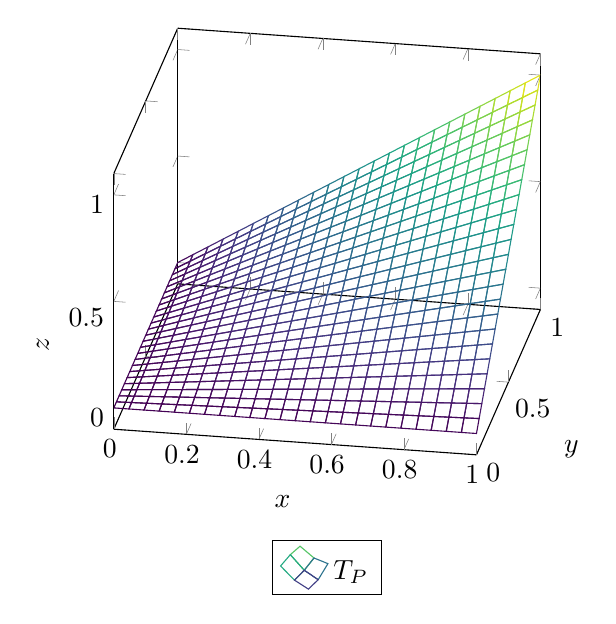
\begin{tikzpicture}
        \begin{axis}[
            width=7cm,  % Nastavte požadovanou šířku grafu
            height=7cm, % Nastavte požadovanou výšku grafu
            xlabel=$x$,
            ylabel=$y$,
            zlabel=$z$, % Popisek osy z
            domain=0:1, % Rozsah hodnot x
            y domain=0:1, % Rozsah hodnot y
            colormap/viridis, % Barevná mapa (nastavitelná)
            view={10}{30}, % Náhled na graf (úhel pohledu)
            legend style={at={(0.5,-0.2)}, anchor=north}
        ]
        
     \addplot3 [surf, shader=interp, mesh] {x*y};
     \legend{$T_P$}
        \end{axis}
    \end{tikzpicture}\\
    \\
    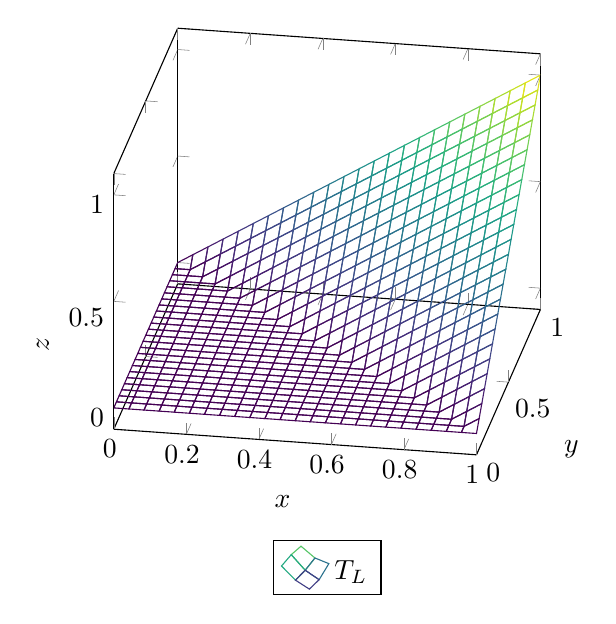
\begin{tikzpicture}
        \begin{axis}[
            width=7cm,  % Nastavte požadovanou šířku grafu
            height=7cm, % Nastavte požadovanou výšku grafu
            xlabel=$x$,
            ylabel=$y$,
            zlabel=$z$, % Popisek osy z
            domain=0:1, % Rozsah hodnot x
            y domain=0:1, % Rozsah hodnot y
            colormap/viridis, % Barevná mapa (nastavitelná)
            view={10}{30}, % Náhled na graf (úhel pohledu)
            legend style={at={(0.5,-0.2)}, anchor=north}
        ]
        
     \addplot3 [surf, shader=interp, mesh] {max(x+y-1,0)};
     \legend{$T_L$}
        \end{axis}
    \end{tikzpicture}
    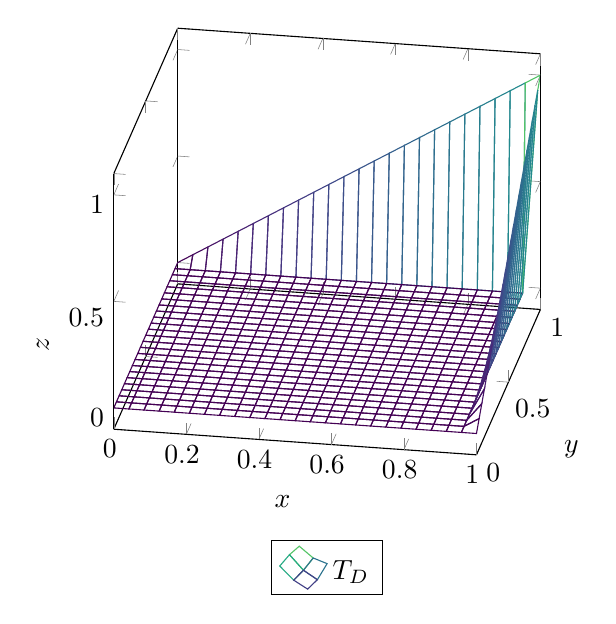
\begin{tikzpicture}
        \begin{axis}[
            width=7cm,  % Nastavte požadovanou šířku grafu
            height=7cm, % Nastavte požadovanou výšku grafu
            xlabel=$x$,
            ylabel=$y$,
            zlabel=$z$, % Popisek osy z
            domain=0:1, % Rozsah hodnot x
            y domain=0:1, % Rozsah hodnot y
            colormap/viridis, % Barevná mapa (nastavitelná)
            view={10}{30}, % Náhled na graf (úhel pohledu)
            legend style={at={(0.5,-0.2)}, anchor=north}
        ]
        
     \addplot3 [surf, shader=interp, mesh] {
                ifthenelse(max(x, y) == 1, min(x, y), 0)
                };
        \legend{$T_D$}
        \end{axis}
    \end{tikzpicture}
\end{graph}

\begin{remark}
    Je zřejmé, že pro každou t-normu T platí
    $$T(1,x)=T(x,1)=x,$$
    $$T(0,x)=T(x,0)=0.$$
\end{remark}
\begin{definition}
\cite{hlinena}
    \begin{itemize}
        \item Pokud pro t-normy $T_1$ a $T_2$ je
        pro každý bod $(x,y) \in [0,1]^2$ splněná nerovnost\\
        $T_1(x,y)\leq ~T_2(x,y),$ znamená to, že $T_1$ je slabší než $T_2$,
        nebo $T_2$ je silnější než $T_1$ a píšeme $T_1\leq T_2$.
        \item  Pokud pro t-normy $T_1$ a $T_2$ platí, že $T_1 \leq T_2$ a
        $T_1 \ne T_2,$ t.j. pokud $T_1 \leq T_2$, ale $T_1(x_0,y_0) <
        T_2(x_0,y_0)$ pro nějaký bod $(x_0,y_0) \in [0,1]^2$, tak $T_1<T_2$.
    \end{itemize}
\end{definition}


Dále je možné zkoumat parametrické třídy t-norem. Mezi známé parametrické třídy patří:
\begin{itemize}
    \item \textbf{Frankovy t-normy:}
    $$T_p^F:(x,y)=\begin{cases} T_M(x,y), & \mbox{pokud }  p = 0,\\ 
                                T_P(x.y), & \mbox{pokud } p = 1,\\
                                T_L(x,y), & \mbox{pokud } p = +\infty,\\
                                log_p(1+\frac{(p^x-1)(p^y-1)}{p-1}), & \mbox{pokud } jinak, 
                                \end{cases}$$
    \item \textbf{Schwarz-Skalarovy t-normy:}
    $$T_p^{SS}:(x,y)=\begin{cases} T_M(x,y), & \mbox{pokud }  p = -\infty,\\ 
                                (x^p+y^p-1)^\frac{1}{p}, & \mbox{pokud }  -\infty < p < 0,\\ 
                                T_P(x.y), & \mbox{pokud } p = 0,\\
                                T_D(x,y), & \mbox{pokud } p = +\infty,\\
                                (max(0, x^p+y^p-1))^\frac{1}{p}, & \mbox{pokud } 0 < p < +\infty, \end{cases}$$
    \item \textbf{Yagerovy t-normy:}
    $$T_p^Y:(x,y)=\begin{cases}  T_D(x,y), & \mbox{pokud } p = 0,\\
                                max(0,1-((1-x)^p+(1-y)^p)^\frac{1}{p} , & \mbox{pokud } 0 < p < +\infty,\\
                                T_M(x,y), & \mbox{pokud } p = +\infty,
                                \end{cases}$$
    \item \textbf{Sugeno-Weberovy t-normy:}
    $$T_p^{SW}:(x,y)=\begin{cases}  T_D(x,y), & \mbox{pokud } p = -1,\\
                                    max(0,\frac{x+y-1+pxy}{1+p}) , & \mbox{pokud } -1 < p < +\infty,\\
                                    T_P(x,y), & \mbox{pokud } p = +\infty.
                                    \end{cases}$$
\end{itemize}

\subsection{Konstrukce triangulárních norem}

Mezi nejznámější konstrukce t-norem patří:
\begin{itemize}
    \item \textbf{Ordinální součet:}
    \begin{definition}
    \cite{hlinena}
        Nech\v t $(T_\alpha)_{\alpha \in A}$ je třída t-norem a
        nech\v t $(]a_\alpha,e_\alpha[)_{\alpha \in A}$ je třída po dvojcích
        disjunktních otevřených podinterval\r u intervalu $[0,1].$ Potom funkce
        \hbox{$T:[0,1]^2\rightarrow [0,1]$} daná předpisem
        $$T(x,y)=\begin{cases} a_\alpha + (e_\alpha - a_\alpha ).T_\alpha (\frac
        {x-a_\alpha}{e_\alpha - a_\alpha}, \frac {y-a_\alpha}{e_\alpha - a_\alpha}),
        &\mbox {pokud $(x,y) \in ]a_\alpha ,e_\alpha [^2$,}
        \\\min(x,y), &\mbox {jinak,} \end{cases}$$
        je t-normou, kterou nazývame {\em ordinálním součtem} sčítanc\r u $\langle a_\alpha ,e_\alpha
        ,T_\alpha \rangle,$ \mbox{$ \alpha \in A.$}
    \end{definition}
    \item \textbf{Aditivní a multiplikativní generování:}
    \begin{definition}
        \cite{hlinena}
        Nech\v t je funkce $f:[0,1] \to [0,\infty]$ spojitá a klesající, přičemž
        $f(1)=0$, potom je předpisem
        $$ T_{<f>}(x,y)=f^{-1}(\min(f(x)+f(y),f(0)))$$
        dána t-norma a funkce $f$ se nazývá aditivní generátor t-normy
        $T_{<f>}.$
        
        Nech\v t je funkce $g:[0,1] \to [0,1]$ spojitá a rostoucí, přičemž
        $g(1)=1$, potom je předpisem
        $$ T^{<g>}(x,y)=g^{-1}(\max(g(x).g(y),g(0)))$$
        dána t-norma a funkce $g$ se nazývá multiplikativní generátor t-normy
        $T^{<g>}.$
    \end{definition}
    \item \textbf{$\varphi$-transformace}
    \begin{definition}
        \cite{hlinena}
        Pokud je $\varphi$ rostoucí bijekce uzavřeného jednotkového intervalu, potom
        předpisem
        $$T_\varphi (x,y)=\varphi ^{-1}(T(\varphi(x),\varphi(y))) \text {pro $(x,y)
        \in [0,1]$}$$
        je dána t-norma, kterou nazýváme $\varphi-${\em transformací t-normy}
        $T.$
    \end{definition}
\end{itemize}

\subsection{Konstrukce spojitých archimedovských triangulárních norem}
\begin{definition}
    T-norma je archimedovská, pokud pro všechny body $(x,y) \in ]0,1[^2$ existuje $n \in N$ takové, že $$x_T^{(n)} < y.$$
\end{definition}
\begin{sentence} (Klement, Mesiar, Pap)
    Triangulární norma T je archimedovská právě, když pro každé $(x,y) \in ]0,1[^2$ je $$\lim_{n \to \infty}x_T^{(n)} = 0$$
\end{sentence}
\begin{sentence} (Klement, Mesiar, Pap)
    Pokud je t-norma T archimedovská, tak pro každé $x \in ]0,1[$ platí $T(x,x) < x.$\\
    Pokud je t-norma spojitá zprava, pak je archimedovská právě, když pro každé $x \in ]0,1[$ platí $T(x,x) < x.$
\end{sentence}

    Součinová a Łukasiewiczova t-norma je typickou představitelkou spojitých archimedovských t-norem.
\begin{sentence} (Klement, Mesiar, Pap)
    Funkce $ T:[0,1]^2 \rightarrow [0,1]$ je
    striktní t-norma právě, když existuje
    rostoucí bijekce $\varphi:[0,1] \rightarrow [0,1]$, taková, že
    $T=(T_P)_\varphi,$ t.j., že
    pro každé $x,y \in [0,1]$ je
    $$T(x,y)=\varphi^{-1}(T_P(\varphi(x),\varphi(y))).$$
\end{sentence}

Spojité archimedovské t-normy se tedy mohou konstruovat pomocí bijekce. Pro konstrukci nespojitých t-norem, které nemají inverzní funkci na celém intervalu, není použití bijekce vhodné. Místo bijekce se pak využívá zevšeobecnění funkce inverzní, t.j. že se k danému zobrazení $f: A \rightarrow B$ přiřazuje prvk\r um z množiny B prvky množiny A, tedy obraz\r um zobrazení $f$ jejich vzory.
\begin{example}
\cite{hlinena}
    Nech\v t je  $f_1:[0,1] \rightarrow [0,1]$  dána předpisem:
    $$f_1(x)=x^2.$$
    Jelikož $f_1$ je bijekce, pro její inverzní a zevšeobecněnou inverzní funkcí
    \newline$f_1^{(-1)}:[0,1] \rightarrow [0,1]$ zřejmě bude platit:
    $$f_1^{(-1)}(x)=f_1^{(-1)}(x)= \sqrt{x}.$$
    Proto složením funkcí $f_1$ a $f_1^{(-1)}$ je
    identita na intervale $[0,1].$
\end{example} 
\begin{graph} Ukázka složení funkcí $f_1^{(-1)} $ a $ f_1$, nebo také zevšeobecnění inverzní funkce.\\

    \resizebox{175pt}{!}{%zde se meni velikost grafu
                \begin{tikzpicture}
                \hspace*{5cm}
                	\begin{axis}[
                        axis lines=middle,
                        xlabel={$x$},
                        ylabel={$y$},
                        xmin=0, xmax=1.1, 
                        ymin=0, ymax=1.1, 
                        xtick={0,0.2,0.4,0.6,0.8,1},
                        ytick={0,0.2,0.4,0.6,0.8,1},
                        legend style={at={(0.5,-0.2)}, anchor=north}
                    ]
                	\addplot[samples = 500,
                            domain=0:1,
                        	smooth,
                        	ultra thick,
                        	blue,] {x^2};
                    
                    \addplot[samples = 500,
                            domain=0:1,
                        	smooth,
                        	ultra thick,
                        	green,] {sqrt(x)};

                    \addplot[samples = 500,
                            domain=0:1,
                        	dashed,
                        	ultra thick,
                        	red,] {x};
                         
                    \legend{$f_1$,
                            $f_1^{(-1)}$,
                            $f_1^{(-1)} \circ f_1$}
                   
                	\end{axis}
                \end{tikzpicture}
            }
\end{graph}

\subsection{Pseudoinverzn\'i funkce}

Ke konstrukci t-norem lze také krom bijekce použít zevšeobecnění pseudoinverzu.
\begin{example}
    \cite{Kolo}
    Nech\v t je dána funkce $f:[0,1]\rightarrow [0,\infty]$, která je klesající, spojitá a $f(1) = 0.$ Obor hodnot této funkce je interval $[0,f(0)]$, přičemž $f(0) \in \textbf{R}$ nebo $f(0) = \infty$, pokud je funkce $f$ shora neohraničená, t.j. pokud $\lim_{x \to 0^+}f(x) = \infty$. Protože $f$ je klesající, existuje k ní inverzní funkce $f^{(-1)}: [0,f(0)] \rightarrow [0,1].$ Po rozšíření funkce na celý interval $[0,\infty]$ tak, že se všem čísl\r um z intervalu $[f(0),\infty]$ přiřadí hodnota 0, vznikne funkce $$f^{-1}: [0,\infty] \rightarrow [0,1],$$
    $$f^{(-1)}(u) = f^{(-1)}(min(u,f(0))),$$
    která se nazývá \textbf{pseudo-inverz} k funkci $f.$
\end{example}
\begin{definition}
    \cite{hlinena}
    Nech\v t je $f:[a,b] \rightarrow [c,d]$ neklesající funkce, pak pro každé $y \in [c,d]$ je předpisem $$f^{(-1)}(y) = sup(x \in [a,b];f(x)<y)$$
    definována pseudoinverzní funkce $f^{(-1)}$ k dané funkci f.
\end{definition}
\begin{definition}
    \cite{hlinena}
    Nech\v t je $f:[a,b] \rightarrow [c,d]$ nerostoucí (nekonstantní) funkce, pak pro každé $y \in [c,d]$ je předpisem $$f^{-1}(y) = sup(x \in [a,b];f(x)>y)$$
    definována pseudoinverzní funkce $f^{(-1)}$ k dané funkci f.
\end{definition}
\begin{sentence} (Hliněná, Biba)
    Nech\v t je $c$ kladné reálné číslo. Potom pro monot\'onní funkci $f:[0,1]\rightarrow
    [0,\infty]$ plat\'i
    $$\left (c\cdot f \right )^{(-1)}(x) = f^{(-1)}\left (\frac {x}{c} \right
    ).$$
\end{sentence}

Generátory nespojitých t-norem tedy zřejmě nemusí být bijekce. Na následujícím příkladu je obdobně, jako v Příkladu 4. ukázka zevšeobecnění inverzní funkce.
\begin{example}
\cite{hlinena}
\begin{enumerate}
    \item Nech\v t je $f_2:[0,1] \rightarrow [0,1]$ dána předpisem:
    $$f_2(x)= \begin{cases} \frac x2, & \mbox {pokud $x \in [0,\frac 12],$}
    \\ \frac 14, & \mbox {pokud $x \in ]\frac 12,\frac 34],$}
    \\ 3.x-2, & \mbox {pokud $x \in ]\frac 34,1]$.}
    \end{cases}$$
    Funkce $f_2$ není injekce, což znamená, že k ní neexistuje inverzní funkce. Na intervale $[0,\frac 12]$ je funkce $f_2$ spojitá a injektivní, proto na daném oboru hodnot $[f(0),f(\frac 12)]$ je
    funkce $f_2^{(-1)}$ totožná s~inverzní funkcí
    $f_{2/[f(0),f(\frac 12)]}^{-1}.$
    Potom pro monot\'oní rozšíření inverzní funkce plat\'i
    $$f_2^{(-1)}(x)= \begin{cases} 2x, & \mbox {pokud $x \in [0,\frac 14],$}
    \\ \frac x3 + \frac 23, & \mbox {pokud $x \in ]\frac 14,1].$}
    \end{cases}$$
    Složení funkcí pak bude vypadat následovně:
    $$g(x)=f_2^{(-1)} \circ f_2(x)=f_2^{(-1)} \left(f_2(x)\right)= \begin{cases} \frac 12,
    & \mbox{pokud $x \in [\frac 12,\frac 34],$}
    \\x, & \mbox {jinak.} \end{cases}$$
    
    \item Nech\v t je $f_3:[0,1] \rightarrow [0,1]$ dána předpisem:
    $$f_3(x)= \begin{cases} 2x, & \mbox {pokud $x \in [0,\frac 14],$}
    \\ \frac x3 + \frac 23, & \mbox {pokud $x \in ]\frac 14,1].$}
    \end{cases}$$
    Funkce $f_3$ je injektivní, takže k ní narozdíl od funkce $f_2$ existuje inverzní funkce. Jenomže funkce $f_3$ není bijektivní, tudíž její inverzní funkce nebude definována na celém intervalu $[0,1]$. 
    Její jediné monot\' onní rozšíření na celý interval $[0,1]$ je dáno předpisem
    $$f_3^{(-1)}(x)= \begin{cases} \frac x2, & \mbox {pokud $x \in [0,\frac 12],$}
    \\ \frac 14, & \mbox {pokud $x \in ]\frac 12,\frac 34],$}
    \\ 3.x-2, & \mbox {pokud $x \in ]\frac 34,1]$.}
    \end{cases}$$
\end{enumerate}
\end{example}
Následující grafy zobrazují zmíněné funkce $f_2$ a $f_3$ a jejich složení s inverzními funkcemi.

\begin{graph} Zobrazení funkcí z Příkladu 6. Modře jsou vyznačeny (zleva) funkce $f_2$ a $f_3$, zeleně jejich zevšeobecněné inverzní funkce a červeně složené funkce $f_2^{(-1)} \circ f_2(x) $~a~$ f_3^{(-1)}\circ ~f_3(x).$\\
     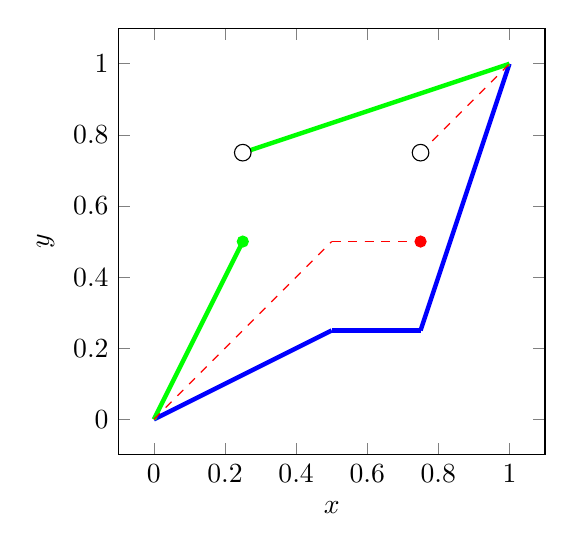
\begin{tikzpicture}
        \begin{axis}[
            width=7cm,  
            height=7cm, 
            xlabel=$x$,
            ylabel=$y$,
            domain=0:1,
            colormap/viridis,
            view={0}{90}, 
        ]
        
        \addplot[domain=0:0.5, ultra thick, samples=100, blue] {x/2};
        \addplot[domain=0.5:0.75, ultra thick, samples=100, blue] {1/4};
        \addplot[domain=0.75:1, ultra thick, samples=100, blue] {3*x-2};

        \addplot[domain=0:0.25, ultra thick, samples=100, green] {2*x};
        \addplot[domain=0.25:1, ultra thick, samples=100, green] {(x/3) + (2/3)};
        \addplot[green, mark=*] coordinates {(1/4, 1/2)};
        \addplot[only marks, mark=*, mark size=3pt, mark options={fill=white}] coordinates {(1/4,3/4)};
        

        \addplot[domain=0:0.5, dashed, samples=100, red] {x}; 
        \addplot[domain=0.5:0.75, dashed, samples=100, red] {1/2};
        \addplot[domain=0.75:1, dashed, samples=100, red] {x};
        \addplot[red, mark=*] coordinates {(3/4, 1/2)};
        \addplot[only marks, mark=*, mark size=3pt, mark options={fill=white}] coordinates {(3/4,3/4)};

        \end{axis}
        \end{tikzpicture}
        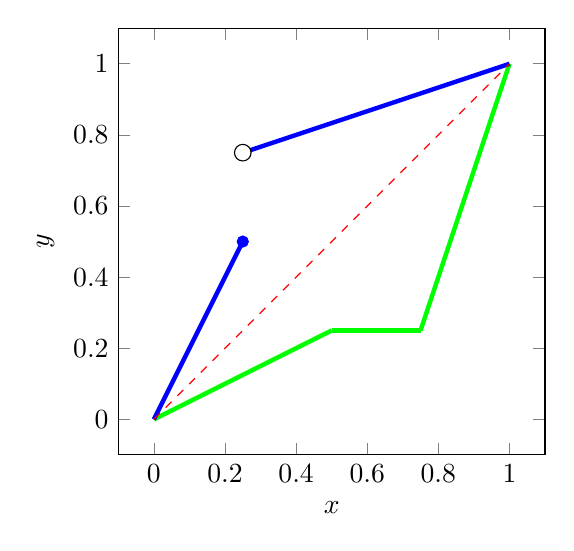
\begin{tikzpicture}
        \begin{axis}[
            width=7cm,  
            height=7cm, 
            xlabel=$x$,
            ylabel=$y$,
            domain=0:1,
            colormap/viridis,
            view={0}{90}, 
        ]
        
        \addplot[domain=0:0.5, ultra thick, samples=100, green] {x/2};
        \addplot[domain=0.5:0.75, ultra thick, samples=100, green] {1/4};
        \addplot[domain=0.75:1, ultra thick, samples=100, green] {3*x-2};

        \addplot[domain=0:0.25, ultra thick, samples=100, blue] {2*x};
        \addplot[domain=0.25:1, ultra thick, samples=100, blue] {(x/3) + (2/3)};
        \addplot[blue, mark=*] coordinates {(1/4, 1/2)};
        \addplot[only marks, mark=*, mark size=3pt, mark options={fill=white}] coordinates {(1/4,3/4)};
        

        \addplot[domain=0:1, dashed, samples=100, red] {x}; 

        \end{axis}
        \end{tikzpicture}
            
\end{graph}

Na Obrázku 7. lze zřejmě pozorovat následující situaci: $$f_2(x)=f_3^{(-1)}\text{ a } f_3(x)=f_2^{(-1)}(x), \text{ takže } (f_2^{(-1)})^{(-1)}(x)=f_2(x) \text{ a }
            (f_3^{(-1)})^{(-1)}(x)=f_3(x).$$
\begin{remark} Na předchozích příkladech bylo naznačeno konstruování pseudoinverzní funkce. Nech\v t je $f:[a,b] \rightarrow [x,d]$ neklesající funkce, lze si pak všimnout určitých poznatk\r u:
    \begin{itemize}
        \item pokud je funkce $f$ bijekce, tak platí $f^{(-1)}(x) = f^{-1}(x),$
        \item  pokud je funkce $f$ rostoucí, její pseudoinverzní funkce je spojitá,
        \item  pro každé $x \in [a,b]$ platí: $f^{(-1)}\circ f(x)\leq x.$
    \end{itemize}
    Nech\v t je $f:[a,b] \rightarrow [x,d]$ nerostoucí funkce:
    \begin{itemize}
        \item pokud je funkce $f$ bijekce, tak platí $f^{(-1)}(x) = f^{-1}(x),$
        \item  pokud je funkce $f$ klesající, její pseudoinverzní funkce je spojitá,
        \item  pro každé $x \in [a,b]$ platí: $f^{(-1)}\circ f(x)\leq x.$
    \end{itemize}
\end{remark}

\begin{sentence} (Klement, Mesiar, Pap)
    Nech\v t je $f:[0,1] \rightarrow [0,\infty]$ klesající funkce
    taková, že $f(1)=0$ a pro všechny $(x,y) \in [0,1]^2$  je splněno
    $$f(x)+f(y) \in H(f) \cup [f(0)^+,\infty].$$
    Potom funkce dvou proměnných $T:[0,1]^2 \rightarrow [0,1]$ dána předpisem
    $$T(x,y)=f^{(-1)}(f(x)+f(y))$$
    je triangulární norma.
\end{sentence}
\begin{sentence}(Klement, Mesiar, Pap)
    Nech\v t je $l:[0,1] \rightarrow [0,1]$ rostoucí funkce
    taková, že $l(1)=1$ a pro všechny $(x,y) \in [0,1]^2$  je splněno
    $$l(x).l(y) \in H(l) \cup [0,l(0)^+].$$
    Potom funkce dvou proměnných $T:[0,1]^2 \rightarrow [0,1],$ dána předpisem
    $$T(x,y)=l^{(-1)}(l(x).l(y)),$$
    je triangulární norma.
\end{sentence}

Pseudoinverzní funkce používají k definici aditivního a multiplikativního generátoru

\begin{definition}
    \cite{hlinena}
    Aditivní generátor t-normy $T$ je klesající funkce
    $f:[0,1] \rightarrow [0,\infty],$ která je zprava-spojitá v~bodě $0,
    f(1)=0$
    a pro všechny $(x,y) \in [0,1]^2$ je splněno
    $$f(x)+f(y) \in H(f) \cup [f(0),\infty],$$
    přitom t-norma $T$ je dána předpisem:
    $$T(x,y)=f^{(-1)}(f(x)+f(y)).$$
\end{definition}
\begin{definition}
    \cite{hlinena}
    Multiplikativní generátor t-normy $T$ je rostoucí funkce
    $l:[0,1] \rightarrow [0,1],$ která je zprava-spojitá v~bodě $0, l(1)=1$
    a pro všechny $(x,y) \in [0,1]^2$ je splněno
    $$l(x).l(y) \in H(l) \cup [0,l(0)],$$
    přitom t-norma $T$ je dána předpisem:
    $$T(x,y)=l^{(-1)}(l(x).l(y)).$$
\end{definition}

\subsection{Fuzzy disjunkce} 
Fuzzy disjunkce vyjadřuje stejně jako fuzzy konjunkce míru spojení dvou či více prvk \r u. Výsledek fuzzy disjunkce je hodnota $x \in [0,1],$ přičemž 0 značí neexistující spojitost mezi prvky a 1 značí, že jsou prvky plně spojeny.
Základní vlastnosti fuzzy disjunkcí jsou:
\begin{enumerate}
    \item \textbf{Soudržnost:}\\
    Pro hodnoty 0 a 1 se fuzzy disjunkce shoduje s klasickou disjunkcí.
    \item \textbf{Kontinuita hodnot:}\\
    Fuzzy disjunkce nepracuje jenom s  ostrými hodnotami „pravda“ a „nepravda“, ale na stupni neurčitosti či specifickým číselném zápisu, který reflektuje stupeň spojení prvk\r u.
   \item \textbf{Monotonie:}\\
    Fuzzy disjunkce je monotonní operace, tedy pokud A$\leq$ B$\leq$ C$\leq$ D, pak A$\lor$B$\leq$ C$\lor$D, což znamená, že s klesajícími vstupními hodnotami klesají i výsledky jejich disjunkce.
\end{enumerate}

\begin{definition}
    \cite{hlinena}
    Neklesající zobrazení $D: [0,1]^2 \rightarrow [0,1]$ se nazývá disjunktor, pokud pro libovolné $a, b \in [0,1]$ platí $$D(a,b) = 1  \text{ pokud }  a = 1, \text{nebo }  b = 1,$$
    $$D(0,0) = 0.$$
\end{definition}

Operace fuzzy disjunkce může být definována různými způsoby, včetně Max-Min disjunkce a Pravd\v epodobnostn\' i disjunkce:
\begin{enumerate}
    \item \textbf{Max-Min disjunkce:}
    Mezi nejtypičtější fuzzy disjunkci patří max-min disjunkce $D_M$.
    $$D_M(A,B) = max(min(\mu_A(x), \mu_B(x)))$$
    kde $\mu_A()x$ a $\mu_B(x)$ jsou příslušnostní funkce množin A a B pro daný prvek $x.$
    \item \textbf{Pravd\v epodobnostn\' i disjunkce:}
    Tato disjunkce je založena na Bayesově teorii pravděpodobnosti a kombinuje informace o pravděpodobnosti spojení A a B:
    $$D_P(A,B) = \frac{\text{Pravděpodobnost spojení } A \text{ a } B}{\text{Pravděpodobnost spojení } A \text{ a } B + \text{Pravděpodobnost jejich průniku}}.$$
\end{enumerate}

Fuzzy disjunkce mohou být konstruovány pomocí triangulárních konorem.

\subsection{Triangul\'arn\'i konormy} 
\label{sec: Triangulární konormy}
Triangulární konormy (zkráceně t-konormy) a t-normy jsou komplementární operace, což znamená, že se vzájemně dopl\v nují a v mnoha případech pak značí operace sobě opačné.
\begin{definition}
    \cite{hlinena}
    Pokud je $T$ t-norma, tak její duální t-konorma $S: [0,1]^2 \rightarrow [0,1]$ je dána předpisem $$S(x,y) = 1 - T(1-x, 1-y).$$
\end{definition}
\begin{definition}
    T-konorma je binární operace na intervalu $[0,1],$ t.j. funkce $S: [0,1]^2 \rightarrow [0,1]$ taková, že pro každé $x, y, z \in [0,1]$ jsou splněny následující axiomy:
    \begin{enumerate}
        \item \textbf{Komutativnost: } $S(x,y) = S(y,x),$
        \item \textbf{Asociativita: } $S(x,S(y,z)) = S(S(x,y),z)$,
        \item \textbf{Monotónnost:} pokud $y \leq z$ pak $T(x, y) \leq T(x, z)$,
        \item \textbf{Okrajová podmínka: } $S(x,0) = x.$
    \end{enumerate}
\end{definition}

Mezi základní triangulární konormy se obdobně (ale komplementárně) jako u t-norem řadí maximová a Łukasiewiczova t-norma, pravděpodobnostní a drastický součet.
\begin{example}
\cite{hlinena}
    \begin{enumerate}
    \item \textbf{Maximová t-konorma} $S_M: [0,1]^2 \rightarrow [0,1]$
    $$S_M(x,y) = max(x,y).$$
    \item \textbf{Pravděpodobnostní součet} $S_P: [0,1]^2 \rightarrow [0,1]$
    $$S_P(x,y) = x+y-x.y.$$
    \item \textbf{Łukasiewiczova t-konorma} $S_L: [0,1]^2 \rightarrow [0,1]$
    $$S_L(x,y) = min(x+y,1).$$
    \item \textbf{Drastický součet} $S_D: [0,1]^2 \rightarrow [0,1]$
    $$S_D:(x)=\begin{cases} max(x,y), & \mbox{pokud  }  min(x,y) = 0,\\ 
    1, &  jinak.  \end{cases}$$
\end{enumerate}
\end{example}

\begin{graph} Maximová t-konorma $S_M$, Pravděpodobnostní součet $S_P$, Łukasiewiczova t-konorma $S_L$, Drastický součet $S_D$.\\

   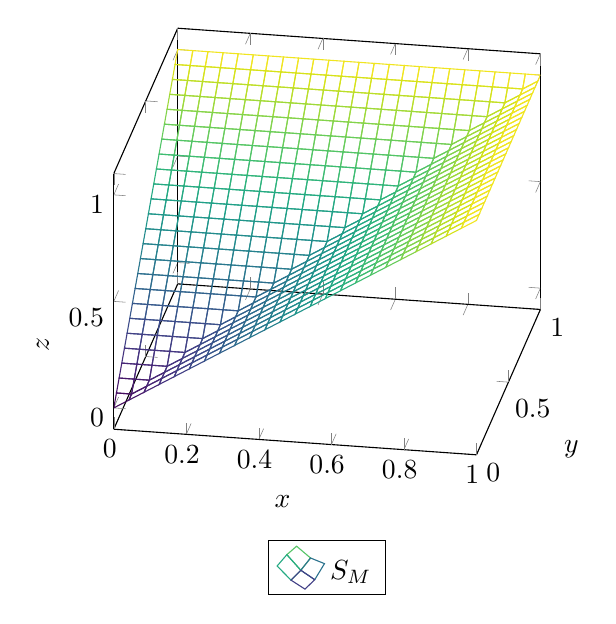
\begin{tikzpicture}
        \begin{axis}[
            width=7cm,  % Nastavte požadovanou šířku grafu
            height=7cm, % Nastavte požadovanou výšku grafu
            xlabel=$x$,
            ylabel=$y$,
            zlabel=$z$, % Popisek osy z
            domain=0:1, % Rozsah hodnot x
            y domain=0:1, % Rozsah hodnot y
            colormap/viridis, % Barevná mapa (nastavitelná)
            view={10}{30}, % Náhled na graf (úhel pohledu)
            legend style={at={(0.5,-0.2)}, anchor=north}
        ]
        
         \addplot3 [surf, shader=interp, mesh] {max(x,y)};
         \legend{$S_M$}
        \end{axis}
    \end{tikzpicture}
    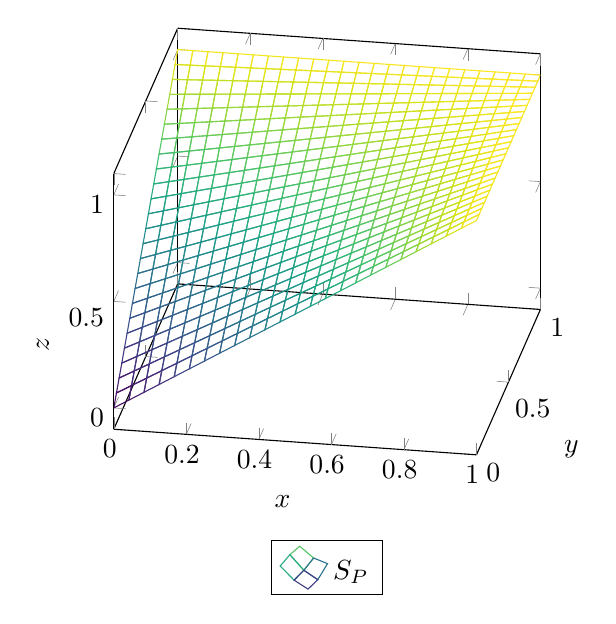
\begin{tikzpicture}
        \begin{axis}[
            width=7cm,  % Nastavte požadovanou šířku grafu
            height=7cm, % Nastavte požadovanou výšku grafu
            xlabel=$x$,
            ylabel=$y$,
            zlabel=$z$, % Popisek osy z
            domain=0:1, % Rozsah hodnot x
            y domain=0:1, % Rozsah hodnot y
            colormap/viridis, % Barevná mapa (nastavitelná)
            view={10}{30}, % Náhled na graf (úhel pohledu)
            legend style={at={(0.5,-0.2)}, anchor=north}
        ]
        
     \addplot3 [surf, shader=interp, mesh] {x+y-x*y};
     \legend{$S_P$}
        \end{axis}
    \end{tikzpicture}\\
    \\
    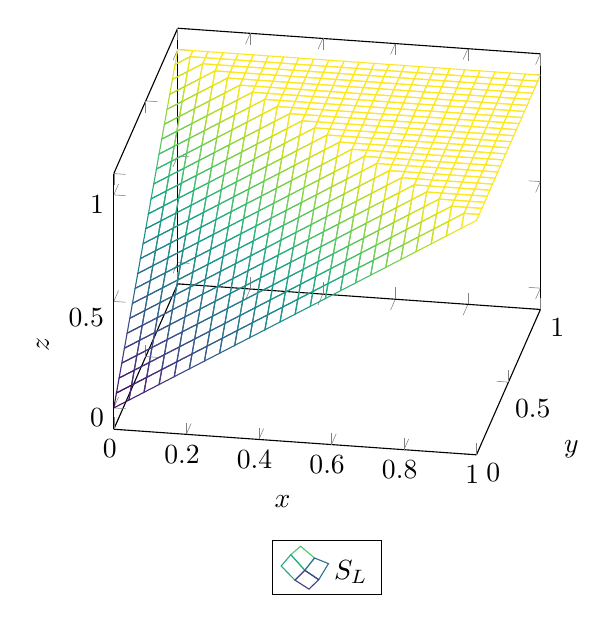
\begin{tikzpicture}
        \begin{axis}[
            width=7cm,  % Nastavte požadovanou šířku grafu
            height=7cm, % Nastavte požadovanou výšku grafu
            xlabel=$x$,
            ylabel=$y$,
            zlabel=$z$, % Popisek osy z
            domain=0:1, % Rozsah hodnot x
            y domain=0:1, % Rozsah hodnot y
            colormap/viridis, % Barevná mapa (nastavitelná)
            view={10}{30}, % Náhled na graf (úhel pohledu)
            legend style={at={(0.5,-0.2)}, anchor=north}
        ]
        
     \addplot3 [surf, shader=interp, mesh] {min(x+y,1)};
     \legend{$S_L$}
        \end{axis}
    \end{tikzpicture}
    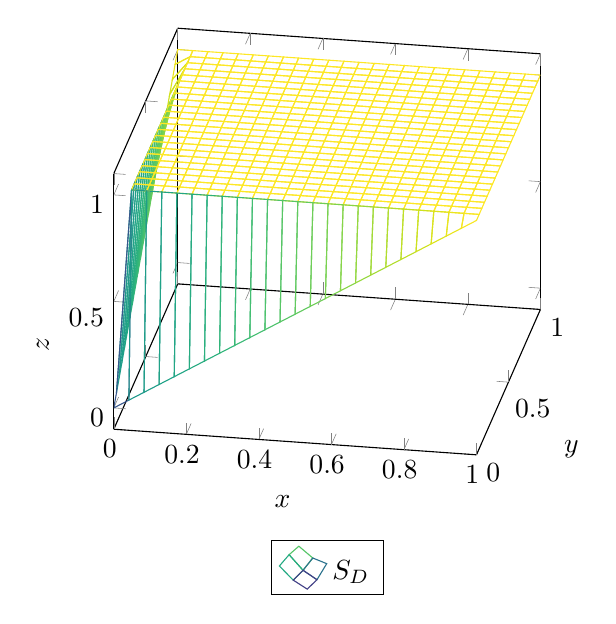
\begin{tikzpicture}
        \begin{axis}[
            width=7cm,  % Nastavte požadovanou šířku grafu
            height=7cm, % Nastavte požadovanou výšku grafu
            xlabel=$x$,
            ylabel=$y$,
            zlabel=$z$, % Popisek osy z
            domain=0:1, % Rozsah hodnot x
            y domain=0:1, % Rozsah hodnot y
            colormap/viridis, % Barevná mapa (nastavitelná)
            view={10}{30}, % Náhled na graf (úhel pohledu)
            legend style={at={(0.5,-0.2)}, anchor=north}
        ]
        
     \addplot3 [surf, shader=interp, mesh] {
                ifthenelse(min(x, y) == 0, max(x, y), 1)
                };
        \legend{$S_D$}
        \end{axis}
    \end{tikzpicture}
\end{graph}

\subsection{Fuzzy implikace} 

Fuzzy implikace patří mezi nejd\r uležitější fuzzy pojmy a díky takovým spojením výrok\r u je možné mnohem jednodušeji popsat lidské vyjadřování matematicky. Implikace se v obecném jazyce vyjadřuje mnoha zp\r usoby, nejtypičtěji pak slovním spojením \textit{když-tak}. Fuzzy implikace je, podobn\v e jako p\v redchoz\'i logick\'e spojky, monot\'onn\'im roz\v s\'i\v ren\'im klasick\'e implikace.
\begin{definition}
    Zobrazení $I: [0,1]^2 \rightarrow [0,1] $ se nazývá implikátor, pokud
    \begin{itemize}
        \item $I$ je nerostoucí ve svojí první souřadnici,
        \item $I$ je neklesající ve svojí druhé souřadnici,
        \item $I(1,0) = 0, I(0,0) =  I(0,1) = I(1,1) = 1.$
    \end{itemize}
\end{definition}

Modelov\'an\'i fuzzy implikace je ale o něco složitější, než modelov\'an\'i dříve zmíněných logických spojek. Fuzzy konjunkce se modelují pomocí t-norem, disjunkce pomocí t-konorem a negace pomocí fuzzy negátor\r u. Tyto spojky pak mohou být využity pro modelaci fuzzy implikace. Zřejmě jsou následující logické formule tautologicky ekvivalentní: $$ p\implies q, \mbox{   } \neg p \vee q, \mbox{   } \neg p\vee (p\wedge q) .$$ Lze tedy spojit informace o modelov\'an\'i logických spojek a jejich vzájemných ekvivalentních \' upravách pro tvorbu fuzzy implikátoru: $$I(x,y)=S(N(x),y)\text{ neboli S-implikátory},$$
$$I(x,y)=S(N(x),T(x,y)) \text{ neboli Q-implikátory}.$$\\
Pokud je $N$ silná fuzzy negace, pak se $I$ nazývá silná fuzzy implikace nebo také S-implikace. Mimo to pokud je $I (S,N)-$implikace generována t-konormou $S$ a negátorem $N$, označuje se indexem $I_{S,N}.$ 

\begin{example}
\cite{hlinena}
Pro základní t-konormy zmíněné v kapitole \ref{sec: Triangulární konormy} a standardní negátor $N_S$ existují následující implikátory, které patří do skupiny $(S,N)-$implikátor\r u:\\
    \vbox{$$ I_{S_M}(x,y)=\max(1-x,y),$$ }
\vbox{$$ I_{S_P}(x,y)=1-x+x.y,$$}
 \vbox{$$ I_{S_L}(x,y)=\min(1-x+y,1),$$}
 $$ I_{S_D}(x,y)=\begin{cases} 1-x,
&\mbox {pokud y=0,} \\y, &\mbox {pokud x=1}, \\
1, &\mbox {jinak.} \end{cases} $$
\end{example}

Pro představu jsou níže představeny grafy implikátorů $I_{S_M}, I_{S_P}, I_{S_L}$ a $I_{S_D}.$
\begin{graph} Uk\' azka implik\' ator\r u.\\
\\
    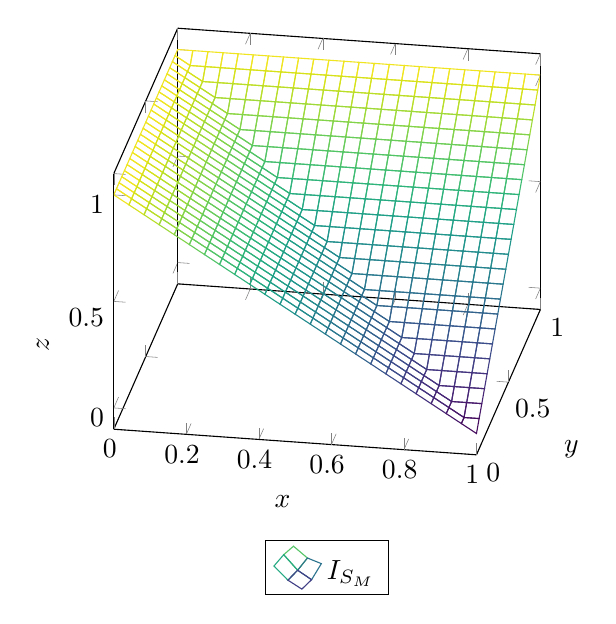
\begin{tikzpicture}
        \begin{axis}[
            width=7cm,  % Nastavte požadovanou šířku grafu
            height=7cm, % Nastavte požadovanou výšku grafu
            xlabel=$x$,
            ylabel=$y$,
            zlabel=$z$, % Popisek osy z
            domain=0:1, % Rozsah hodnot x
            y domain=0:1, % Rozsah hodnot y
            colormap/viridis, % Barevná mapa (nastavitelná)
            view={10}{30}, % Náhled na graf (úhel pohledu)
            legend style={at={(0.5,-0.2)}, anchor=north}
        ]
        
     \addplot3 [surf, shader=interp, mesh] {max(1-x,y)};
        \legend{$I_{S_M}$}
        \end{axis}
    \end{tikzpicture}
    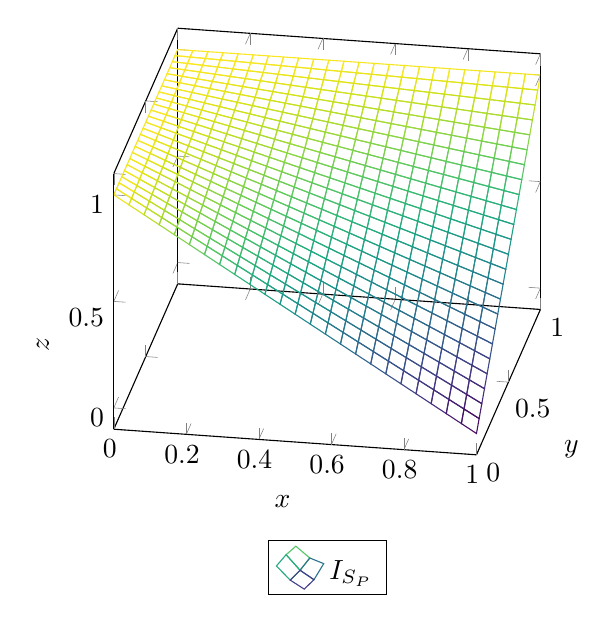
\begin{tikzpicture}
        \begin{axis}[
            width=7cm,  % Nastavte požadovanou šířku grafu
            height=7cm, % Nastavte požadovanou výšku grafu
            xlabel=$x$,
            ylabel=$y$,
            zlabel=$z$, % Popisek osy z
            domain=0:1, % Rozsah hodnot x
            y domain=0:1, % Rozsah hodnot y
            colormap/viridis, % Barevná mapa (nastavitelná)
            view={10}{30}, % Náhled na graf (úhel pohledu)
            legend style={at={(0.5,-0.2)}, anchor=north}
        ]
        
     \addplot3 [surf, shader=interp, mesh] {1-x+x*y};
        \legend{$I_{S_P}$}
        \end{axis}
    \end{tikzpicture}
    
    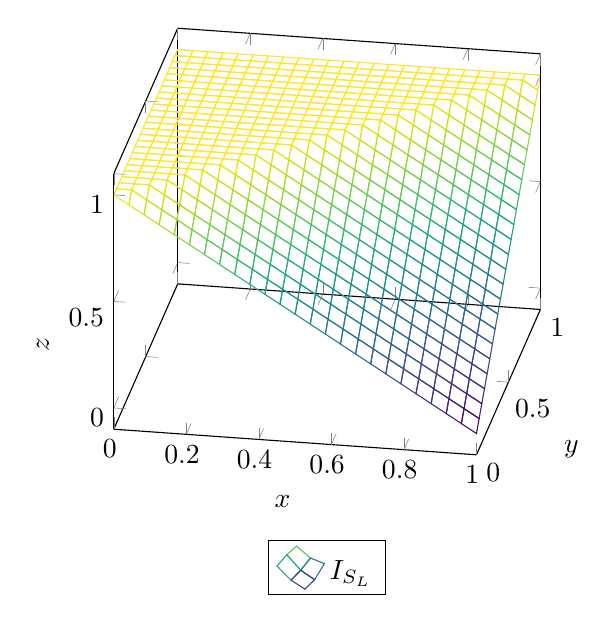
\begin{tikzpicture}
        \begin{axis}[
            width=7cm,  % Nastavte požadovanou šířku grafu
            height=7cm, % Nastavte požadovanou výšku grafu
            xlabel=$x$,
            ylabel=$y$,
            zlabel=$z$, % Popisek osy z
            domain=0:1, % Rozsah hodnot x
            y domain=0:1, % Rozsah hodnot y
            colormap/viridis, % Barevná mapa (nastavitelná)
            view={10}{30}, % Náhled na graf (úhel pohledu)
            legend style={at={(0.5,-0.2)}, anchor=north}
        ]
        
     \addplot3 [surf, shader=interp, mesh] {min(1-x+y,1)};
        \legend{$I_{S_L}$}
        \end{axis}
    \end{tikzpicture}
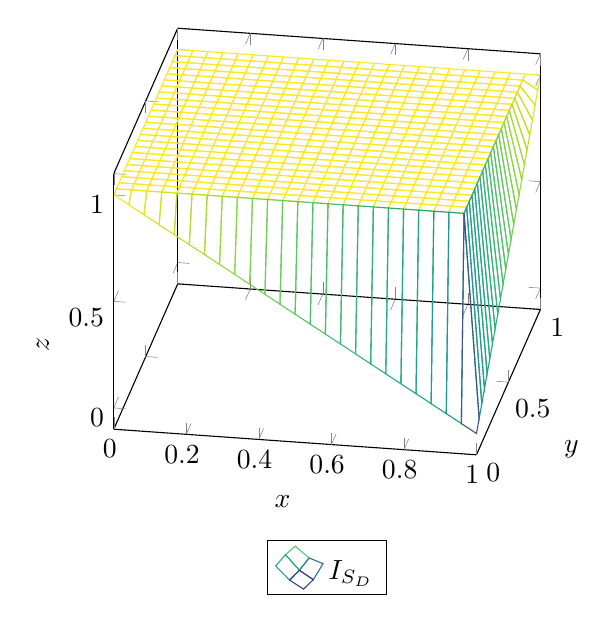
\begin{tikzpicture}
        \begin{axis}[
            width=7cm,  % Nastavte požadovanou šířku grafu
            height=7cm, % Nastavte požadovanou výšku grafu
            xlabel=$x$,
            ylabel=$y$,
            zlabel=$z$, % Popisek osy z
            domain=0:1, % Rozsah hodnot x
            y domain=0:1, % Rozsah hodnot y
            colormap/viridis, % Barevná mapa (nastavitelná)
            view={10}{30}, % Náhled na graf (úhel pohledu)
            legend style={at={(0.5,-0.2)}, anchor=north}
        ]
        
     \addplot3 [surf, shader=interp, mesh] {ifthenelse(y==0,1-x,ifthenelse(x==1,y,1))};
        \legend{$I_{S_D}$}
        \end{axis}
    \end{tikzpicture}

\end{graph}

Mezi nejznámější Q-implikátor patří tzv. Zadeh\r uv implikátor, který staví na $T_M, S_M, N_S$ a má předpis $$I_Z(x,y) = max(1-x, min(x,y)).$$ Po použití $T_L, S_L, N_S$ bude výsledkem klasický S-implikátor založený na $S_M.$
Mezi nejpoužívanější rozšíření klasické implikace na interval $[0,1]$ je \textit{reziduální operátor} $R_T$ pro danou zleva-spojitou t-normu T: $$ R_T(x,y)=\sup(z \in [0,1]; T(x,z) \leq y).$$

Ve vícehodnotové logice na rozdíl od bivalentní logiky nemusí platit tvrzení, že jsou si implikátory $I_T$ a $R_T$ rovny. Následující příklad je toho d\r ukazem.
\begin{example} Pro zleva spojité t-normy $T_M, T_P$ a $T_L$ pak mohou vzniknout následující reziduální implikátory:
    \cite{hlinena}\\
     $$ R_{T_M}(x,y)=\begin{cases} 1, &\mbox {ak $x\leq y$,} \\y, &\mbox{jinak,} \end{cases} $$
    (Göddelov implik\' ator)
     $$ R_{T_P}(x,y)=\min \left (\frac yx,1 \right ),$$
    (Goguenov implikátor)
     $$ R_{T_L}(x,y)=\min(1-x+y,1).$$
    (\L{}ukasiewiczov implikátor)\\
\end{example}
\begin{definition}
\cite{hlinena}
Klasický implik\'ator $I:[0,1]^2 \rightarrow [0,1]$ spl\v nuje:
\begin{enumerate}
\item[(NP)] levý princip neutrality, pokud
$$I(1,y)=y; ~~~~y \in [0,1],$$
\item[(EP)] princip z\'aměny, pokud
$$I(x,I(y,z))=I(y,I(x,z)) \mbox{  pro ka\v zd\'e   } x,y,z \in [0,1],$$
\item[(IP)] princip identity, pokud
$$I(x,x) = 1; ~~~ x \in [0,1], $$
\item[(OP)] vlastnost uspořádání
$$x \leq y \iff I(x,y) =1; ~~~ x,y \in [0,1],$$
\item[(CP)] kontrapozitivitu vzhledem na dan\'y neg\'ator $N$, pokud
$$ I(x,y)=I(N(y),N(x)); ~~~ x,y \in [0,1].$$
 {\item[(LI)] z\'akon přenosu  vzhledem na  t-normu $T$, pokud
$$I(T(x, y), z) = I(x, I(y, z)); ~~~ x,y,z \in  [0, 1].$$
\item[(WLI)]  slab\'y z\'akon přenosu vzhledem na komutativní a
rostoucí funkci $F:
[0,1]^2 \to [0, 1]$, pokud
$$I(F(x, y), z) = I(x, I(y, z)); ~~~  x,y,z \in  [0, 1].$$}
\end{enumerate}
\end{definition}
Ne všechny fuzzy implikátory ale spl\v nují všechny výše uvedené vlastnosti. Např. S-implikátory spl\v nují pouze $(NP)$ a $(EP)$, reziduální implikátor zase spl\v nuje pouze $(NP)$ a $(OP).$ Na základě takových vlastností lze implikátory rozdělit do skupin (např. (S,N)-implikátory, R-implikátory nebo Q-impkilátory), se kterými pak lze dále pracovat.
\subsection{Konstrukce fuzzy implikátor\r u}

Většina konstruktor\r u je ve fuzzy logice modelována pomocí t-norem. Konstrukce nových t-norem, tedy nových konjunktor\r u, je naznačena v předchozích kapitolách. Při konstruování implikátor\r u lze použít podobný postup.

\begin{definition}
    Nech\v t je $\varphi:[0,1] \rightarrow [0,1]$  rostoucí
    bijekce a množina všech takových bijekcí Nech\v t je {\em B.} Nech\v t je funkce
    $I:[0,1]^2\rightarrow [0,1]$ 
    implikátor.
    Pak je funkce
    $$I_\varphi(x,y)=\varphi^{-1}(I(\varphi (x), \varphi (y)))$$
    $\varphi-${\em transformací implikátoru} $I.$ Implikátor se nazývá
    {\em totálně invariantní,} pokud pro libovolnou funkci $\varphi \in B$ platí $I_\varphi=I.$\\
\end{definition}

\begin{sentence}(Baczy\v nski, Drewniak)
    Nech\v t $\varphi \in B$, potom pro libovolný implikátor $I: [0,1]^2 \rightarrow [0,1]$ je $\varphi$-transformace $I_\varphi$ také implikátor.
\end{sentence}

Generování implikátor\r u lze rozdělit do tří tříd. Yager popsal první dvě třídy, tedy f-generované a g-generované implikátory. Za popsání  h-generovaných implikátor\r u, tedy poslední třídy, si připisuje zásluhy Balasubramaniam Jayram. Následně jsou všechny třídy představeny.

\begin{sentence}(Yager) 
Pokud je $f: [0,1] \to [0,\infty]$ klesající a spojitá funkce,
přičemž $f(1) = 0,$ potom je funkce $I: [0,1]^2 \to [0,1],$ dána předpisem
$$I(x,y) = f^{-1}(x \cdot f(y)), \mbox {   } x, y \in [0,1],$$
fuzzy implikátor (pričemž $0 \cdot \infty = 0$). \\
\end{sentence}

\begin{example}
    \cite{hlinena}
    Konstrukce f-generovaných implikátor\r u m\r uže vypadat následovně.
    Pokud by byl použit aditivní generátor součinové t-normy $T_P,$ tedy 
    pokud $f(x) = - \log x,$ výsledkem bude Yager\r uv implikátor:
    $$I_{YG}(x,y)= \begin{cases} 1,
    &\mbox {pokud $x=0$ a $y=0,$} \\
    y^x, &\mbox {jinak.}
    \end{cases}$$
\end{example}
\begin{remark}
    V předchozím příkladu se nejednalo o S-implikátor ani o R-implikátor. To však neplatí v každém případě f-generovaných implikátor\r u.
\end{remark}


\begin{sentence}(Yager) 
Pokud je $g: [0,1] \to [0,\infty]$ klesající a spojitá funkce,
přičemž $g(1) = 0,$ potom je funkce $I: [0,1]^2 \to [0,1],$ dána předpisem
$$I(x,y) = g^{(-1)}\left (\frac 1x \cdot g(y)\right ), \mbox {   } x, y \in [0,1]$$
fuzzy implikátor (pričemž $\frac{1}{0} = \infty, 0 \cdot \infty = 0$). \\
\end{sentence}
\begin{example}
    \cite{hlinena}
    Pokud by byl použit aditivní generátor pravděpodobnostního součtu $S_P,$ tedy 
    pokud $g(x) = - \log (1- x),$ dostaneme následující fuzzy implikátor:
    $$I_{YG}(x,y)= \begin{cases} 1,
    &\mbox {pokud $x=0$ a $y=0,$} \\
    1-(1-y)^x, &\mbox {jinak.}
        \end{cases}$$
\end{example}
\begin{remark}
    Opět se v předchozím příkladu se nejednalo o S-implikátor ani o R-implikátor. To však také neplatí v každém případě g-generovaných implikátor\r u.
\end{remark}

\begin{sentence}(Balasubramaniam) 
Pokud je $h: [0,1] \to [0,\infty]$ klesající a spojitá funkce,
přičemž $h(1) = 0,$ potom je funkce $I: [0,1]^2 \to [0,1],$ dána předpisem
$$I(x,y) = h^{(-1)}(x \cdot h(y)), \mbox {   } x, y \in [0,1]$$
fuzzy implikátor. \\
\end{sentence}
\begin{example}
    Pokud by byl jako  $h-$generátor funkce $h_n(x) = 1- \frac {x^n}{n}, n
    \in N,$ výsledkem budou následující fuzzy implikátory:
    $$I_n(x,y) = \min \left ( (n - n \cdot x + x \cdot y^n)^{\frac 1n}, 1\right
    ),$$
    kter\'e jsou $S-$implikátory.
\end{example}
\begin{remark}
    Pro h-negátory platí, že $I_{h_1} = I_{h_2}$ právě když $h_1 = h_2.$
\end{remark}

Všechny třídy generátor\r u jsou, stejně jako v případě spojitých aditivních generátor\r u, jednoznačně dané s proměnlivou kladnou konstantou.

Jednotlivé třídy fuzzy implikátor\r u jse označují následovně:
\begin{itemize}
\item ${\cal I}_{F, \infty}- f-$generované implikátory s $f(0) = \infty,$ 
\item ${\cal I}_{F, \kappa}- f-$generované implikátory s $f(0) < \infty,$ 
\item ${\cal I}_{F} = {\cal I}_{F, \infty} \cup{\cal I}_{F, \kappa}, $
\item ${\cal I}_{G, \infty} - g-$generované implikátory s $g(1) = \infty,$ 
\item ${\cal I}_{G, \kappa} - g-$generované implikátory s $g(1) < \infty,$ 
\item ${\cal I}_{G}={\cal I}_{G, \infty} \cup{\cal I}_{G, \kappa},$ 
\item ${\cal I}_{H, O} - h-$generované implikátory s $h(1) = 0,$ 
\item ${\cal I}_{H, E} - h-$generované implikátory s $g(1) >0,$ 
\item ${\cal I}_{H}= {\cal I}_{H, O} \cup {\cal I}_{H, E}.$ 
\end{itemize} 



\begin{table}[ht!]
    \caption{Vztahy mezi jedlotlivými třídami implikátor\r u\cite{hlinena}}
    \centering 
    \begin{tabular}{|c|c|c|}
    \hline
     $\cup$ & $S-$implikátory & $R-$implikátory\\
    \hline
    ${\cal I}_{F, \infty} = {\cal I}_{G, \infty}$   & $ \emptyset$ & $\emptyset$ \\
    \hline
    ${\cal I}_{F, \kappa} = {\cal I}_{H, O}$   &  ${\cal I}_{F, \kappa}$ &
    $\emptyset$ \\
    \hline
    ${\cal I}_{G, \kappa} = {\cal I}_{H, O}$   &  $\emptyset$ &
    $R_{T_L,}$ \\
    \hline
    ${\cal I}_{H, E}$  &${\cal I}_{H, E}$ &  $\emptyset$\\
    \hline
    \end{tabular}
\end{table}

\begin{example}
    Nech\v t jsou $f_1, f_2, f_3:[0,1] \rightarrow [0,
\infty]$ funkce dan\'e předpisy:
\begin{itemize}
\item $f_1(x)=\begin{cases} 1-x,  &\mbox{pokud $x \leq 0.5$},\\
0.5-0.5x,   &\text{jinak}, \end{cases}$
\item $f_2(x)= \frac{1}{x} -1,$
\item $f_3(x)= -\ln(x).$
\end{itemize}

Je d\r uležité zmínit, že jsou všechny tři funkce klesající. Pro $f_1^{(-1)}, f_2^{(-1)},
f_3^{(-1)}$ pak platí:
\begin{itemize}
\item $f_1^{(-1)}(x)=\begin{cases}  1-2x,       &\mbox{pokud $x \leq 0.25$},\\
0.5,                  &\mbox{pokud $0.25<x \leq 0.5$},\\
1-x,                  &\text{jinak,} \end{cases} $
\item $f_2^{(-1)}(x)=\min \left \{ \frac{1}{1+x},1 \right \},$
\item $f_3^{(-1)}(x)=\min \{ e^{-x},1 \}.$
\end{itemize}
Pro  funkce $f_1, f_2, f_3$ potom lze dostat nasledující implik\'atory:
\begin{itemize}
\item $I_{f_1}(x,y)=\begin{cases}  1,      &\mbox{pokud $x \leq y$}, \\
1-2x+2y,       &\mbox{pokud $x \leq 0.5, y<0.5, x-y \leq 0.25, x > y$}, \\
0.5,       &\mbox{pokud $x \leq 0.5, y<0.5, x-y>0.25$}, \\
0.5 ,      &\mbox{pokud $x>0.5, y<0.5, x \leq 2y$}, \\
0.5+y-0.5x,       &\mbox{pokud $x>0.5, y<0.5, x>2y$}, \\
1-x+y,       &\mbox{pokud $x>0.5, y \geq 0.5,$} \end{cases}$
\item $I_{f_2}(x,y)= \begin{cases} 1,      &\mbox{pokud $x \leq y$}, \\
  \frac{1}{\frac{1}{y} - \frac{1}{x} + 1},     &\text{jinak}, \end{cases} $
\item $I_{f_3}(x,y)= \begin{cases} 1,    &\mbox{pokud $x \leq y$}, \\
  \frac{y}{x},   & \mbox{jinak.} \end{cases}$
\end{itemize}
\end{example}

Dalším typem generovaných implikátor\r u jsou $I^g$ implikátory. Narozdíl od $I_f$ implikátor\r u jsou ale generovány rostoucími funkcemi.

\begin{sentence}(Smutn\'a)\\
    Nech\v t je  $g:[0,1]\rightarrow [0,\infty]$ rostoucí funkce takov\'a, \v ze $g(0)=0$. 
    Potom funkce $I^g(x,y):[0,1]^2 \rightarrow [0,1]$ dan\'a předpisem
    \begin{equation}\label{g}
    I^g(x,y)=g^{(-1)}(g(1-x)+g(y)),
    \end{equation}
    je fuzzy implik\'ator.\\
\end{sentence}

\begin{example}
\cite{hlinena}
    Nech\v t jsou $g_1, g_2:[0,1] \rightarrow [0,\infty]$ 
    dan\'e předpisy:
    \begin{itemize}
    \item $g_1(x)=\begin{cases}  x,    &\mbox{pokud $x \leq 0.5$}, \\
    0.5+0.5x,      &\text{jinak,} \end{cases}$
    \item $g_2(x)=-\ln(1-x).$
    \end{itemize}
    Obě dvě funkce $g_1$ a $g_2$ josu rostoucí.
    Pro jejich pseudo-inverzn\'i funkce  $g_1^{(-1)}$ a $g_2^{(-1)}$ plat\'i:
    \begin{itemize}
    \item $g_1^{(-1)}(x)=\begin{cases} x, &\mbox{pokud $x \leq 0,5$}, \\
    0,5,   &\mbox{pokud $0,5 < x \leq 0,75$}, \\
    2x-1,   &\mbox{pokud $0,75 < x \leq 1$}, \\
    1,   &\mbox{pokud $1 < x$}, \end{cases}$
    \item $g_2^{(-1)}(x)=1-e^{-x} ~ \mbox{pro $x \in [0, \infty]$}.$
    \end{itemize}
    Potom se pro funkce $g_1$ a $g_2$ modelují nasleduj\'icí implik\'atory:
    \begin{itemize}
    \item $I^{g_1}(x,y)=\begin{cases}  1-x+y,      &\mbox{pokud $x \geq 0.5, y \leq 0.5, x-y \geq 0.5$}, \\
    0.5,      &\mbox{pokud $x \geq 0.5, y \leq 0.5, 0.25 \leq x-y < 0.5$}, \\
    1-2x+2y,      &\mbox{pokud $x \geq 0.5, y \leq 0.5, x-y < 0.25$}, \\
    \min(1-x+2y,1),       &\mbox{pokud $x < 0.5, y \leq 0.5$}, \\
    \min(2-2x+y,1),       &\mbox{pokud $x \geq 0.5, y>0.5$}, \\
    1,       &\mbox{pokud $x < 0.5, y > 0.5,$} \end{cases}$
    \item $I^{g_2}(x,y)=1-e^{\ln(x(1-y))}=1-x+xy.$
    \end{itemize}
\end{example}

\begin{sentence}
\cite{hlinena}
    Nech\v t je $c$ kladn\'a konstanta a $g:[0,1] \to [0,\infty]$
    rostoucí  funkce. Potom implik\'atory $I^g$ a $I^{c \cdot g}$,
    které jsou zalo\v zen\'e na  funkcích $g$ a $c \cdot g$, jsou
    identick\'e.
\end{sentence}
